\chapter{FHTBoost: A twodimensional component-wise gradient boosting algorithm for survival data}
\label{ch:FHTboost}
In this chapter, we propose a component-wise boosting algorithm for fitting the inverse Gaussian first hitting time (FHT) model (section \ref{sec:FHT} and onward) to survival data.
We work with survival data sets with $N$ observations,
\begin{equation}\label{eq:data-fhtboost}
    D=(\x_i,\z_i,t_i,d_i)_{i=1}^N.
\end{equation}
Here $t_i$ is a possibly right-censored event time, $d_i$ is an indicator variable which is 1 if $t_i$ is an actually observed event time, and 0 if it is right-censored.
For simplicity, we sometimes denote the response data
\begin{equation*}
    y_i=(t_i,d_i).
\end{equation*}
Further, $\x_i$ and $\z_i$ are covariate vectors that will be related to the inverse Gaussian parameters $y_0$ and $\mu$, respectively.
$\x_i$ is defined as
\begin{equation}
    \x_i=(x_{i,1},x_{i,2},\ldots,x_{i,p_1}),
\end{equation}
with $p_1$ number of covariates, and $\z_i$ is defined as
\begin{equation}
    \z_i=(z_{i,1},z_{i,2},\ldots,z_{i,p_2}),
\end{equation}
with $p_2$ number of covariates.
The dimensions of the matrices, $p_1$ and $p_2$, can be any size, however our motivating setting is a combination of a high-dimensional $p_1$, typically gene data, and a low-dimensional $p_2$, i.e. clinical data. 
There are theoretical arguments for this particular combination of the high and low-dimensional vectors and parameters, which we have discussed earlier in subsection \ref{subsec:FHT-combine}.
Before describing the algorithm in detail, we explain the necessary parts and expressions that will be used in the algorithm.

\section{Structure of the additive predictors}
The first-hitting-time model with Wiener processes, as shown, leads to lifetimes that follow a parameterization of the inverse Gaussian.
Hence its log likelihood depends on $y_0$, $\mu$, with $\sigma$ set to 1 to avoid overparameterization (see subsection \ref{subsec:overdetermined} for reasoning).
Given a data set $D$ \eqref{eq:data-fhtboost}, the log-likelihood of the parameters is
\begin{align*}
\begin{split}
    l(y_0,\mu|D)=\sum_{i=1}^N&d_i\p*{\ln y_0-\frac{1}{2}\ln\p*{2\pi\ti^3}-\frac{\p*{\mu\ti+y_0}^2}{2\ti}} \\
    &+
    (1-d_i)\ln\p*{\Phi\p*{\frac{\mu\ti+y_0}{\sqrt{\ti}}}-\exp\p*{-2y_0\mu}\Phi\p*{\frac{\mu\ti-y_0}{\sqrt{\ti}}}}.
\end{split}
\end{align*}
We denote the $K=2$ distribution parameters as
\begin{equation*}
    \btheta=(\theta_1,\theta_2)^T=(y_0,\mu).
\end{equation*}
We wish to use a similar setup as the GAMLSS (see subsection \ref{subsec:GAMLSS}) to model these parameters.
We will therefore model the parameters in $y_0$ and $\mu$ through additive predictors $\eta_1$ and $\eta_2$, respectively.
We relate the additive predictors to covariates, and further relate the additive predictors to the parameters by their usual link functions, i.e. the log link for $y_0$ (to ensure it is positive) and the identity link for the drift $\mu$.
In FHT regression, the additive predictors are typically \textit{linear} predictors \citep{leewhitmore2006}, and we also use this structure.
We let the additive predictors for an individual $i$ be defined as
\begin{equation}\label{eq:eta1}
    \eta_{1,i}\coloneqq \ln(y_{0,i})=\bbeta^T \x_i=\beta_{0}+\sum_{j=1}^{p_1}x_{i,j}\beta_j
\end{equation}
and
\begin{equation}\label{eq:eta2}
    \eta_{2,i}\coloneqq \mu_{i}=\bgamma^T \z_i=\gamma_{0}+\sum_{j=1}^{p_2}z_{i,j}\gamma_j,
\end{equation}
and we denote the vector containing both as $\boldeta_i=\left(\eta_{1,i},\eta_{2,i}\right)$.
We are going to estimate the additive predictors by gradient boosting, and specifically by estimating the $\beta_j$ and $\gamma_j$ parameters.
In choosing a linear structure for the additive predictors we also choose base learners in the boosting algorithm which allow for this.
We first derive the partial derivatives of the log-likelihood, which will be used to calculate the generalized residuals in each boosting iteration.

\section{Loss function and its partial derivatives}
Since we assume we have observations from a probability distribution, we use the negative of the corresponding log likelihood as our loss function \citep{mayr14a}.
Given the estimated additive predictor $\hat{\boldeta}_i$ for an observation $D_i=(\x_i,\z_i,t_i,d_i)$ from data set D \eqref{eq:data-fhtboost}, we calculate the corresponding estimated distribution parameters by transforming the additive predictors via the inverse of their link functions.
Thus,
\begin{equation}
    \hat{y}_{0,i}=\hat{\theta}_{1,i}=g_1^{-1}(\hat{\eta}_{1,i})=\exp(\hat{\eta}_{1,i}),
\end{equation}
and
\begin{equation}
    \hat{\mu}_i=\hat{\theta}_{2,i}=g_2^{-1}(\hat{\eta}_{2,i})=\hat{\eta}_{2,i}.
\end{equation}
For an observation $y_i$ in \eqref{eq:data-fhtboost}, and estimated parameters $\hat{\btheta}_i=\left(\hat{y}_{0,i},\hat{\mu}_i\right)$ for this observation, we calculate the loss as
\begin{equation*}
    \rho(y_i,\hat{\btheta}_i)=-l(\hat{y}_{0,i},\hat{\mu}_i|D_i).
\end{equation*}
This means that as a function of the additive predictors, the loss function for an observation $i$ is
\begin{equation*}
    \rho(y_i,\hat{\boldeta}_i)=-l(\exp(\hat{\eta}_{1,i}), \hat{\eta}_{2,i}),
\end{equation*}
where $l$ again is the log-likelihood.
To use the gradient boosting algorithm, we need to compute the negative gradient of the loss function, i.e., the negative of the derivative. 
The negative partial derivative of the loss function is just the partial derivative of the log-likelihood function, i.e. the negatives cancel out.
The partial derivative for $y_0$ is
\begin{equation}\label{eq:partial-deriv-y0}
%\begin{split}
    -\frac{\partial}{\partial\eta_1}\rho(y_i,\hat{\btheta}_i)=\frac{\partial}{\partial\eta_1}l(\exp(\hat{\eta}_{1,i}), \hat{\eta}_{2,i})=\hat{y}_{0,i}\frac{\partial}{\partial y_0}l(\hat{y}_{0,i}, \hat{\mu}_{i}),
%\end{split}
\end{equation}
where we used the chain rule because $\eta_1=\exp(y_0)$.
The partial derivative for $\mu$ needs no chain rule because the link function is linear, and so it is
\begin{equation}\label{eq:partial-deriv-mu}
    -\frac{\partial}{\partial\eta_2}\rho(y_i,\hat{\btheta}_i)=\frac{\partial}{\partial\eta_2}l(\exp(\hat{\eta}_{1,i}), \hat{\eta}_{2,i})
    =\frac{\partial}{\partial \mu}l(\hat{y}_{0,i}, \hat{\mu}_{i}).
\end{equation}
These partial derivatives turn out to be quite complicated, but we report them here for completeness, in \eqref{eq:full-partial-deriv-y0} and \eqref{eq:full-partial-deriv-mu}.
See Appendix \ref{appendix} for their complete derivation.

\subsection{Partial derivative for $y_0$}
\begin{align}
\label{eq:full-partial-deriv-y0}
\begin{split}
\frac{\partial}{\partial y_0}
l&\left(\hat{y}_{0,i}, \hat{\mu}_i\right) \\
&=
d_i
\p*{
    \frac{1}{\hat{y}_{0,i}}-\frac{\hat{y}_{0,i}+\hat{\mu}_i\ti}{\sigma^2\ti}
}+
(1-d_i)\cdot\\
&
\left[
    \frac{1}{\sqrt{\ti}}
    \phi\left(\frac{\hat{\mu}_i\ti+\hat{y}_{0,i}}{\sqrt{\ti}}\right)
    +2\hat{\mu}_i\exp\p*{-2\hat{y}_{0,i}\hat{\mu}_i}
    \Phi\p*{\frac{\hat{\mu}_i\ti-\hat{y}_{0,i}}{\sqrt{\ti}}}\right.\\
    &+\left.
    \frac{1}{\sqrt{\ti}}
    \exp\left(
        -2\hat{y}_{0,i}\hat{\mu}_i
    \right)
    \phi\left(\frac{\hat{\mu}_i\ti-\hat{y}_{0,i}}{\sqrt{\ti}}
    \right)
\right]\cdot\\
&\left[
    \Phi\left(
        \frac{\hat{\mu}_i t_i + \hat{y}_{0,i}}{\sqrt{t_i}}
    \right)
    -\exp\left(-2\hat{y}_{0,i}\hat{\mu}_i\right)
    \Phi
    \left(
        \frac{\hat{\mu}_i t_i - \hat{y}_{0,i}}{\sqrt{t_i}}
    \right)
\right]^{-1}
\end{split}
\end{align}

\subsection{Partial derivative for $\mu$}
\begin{align}
\label{eq:full-partial-deriv-mu}
\begin{split}
\frac{\partial}{\partial \mu}
l&(\hat{y}_{0,i}, \hat{\mu}) \\
&=
d_i\p*{-\hat{y}_{0,i}+\hat{\mu}\ti}+(1-d_i)\cdot \\
&\left[
\frac{\ti}{\sqrt{\ti}}\phi\p*{\frac{\hat{\mu}\ti+\hat{y}_{0,i}}{\sqrt{\ti}}}+2\hat{y}_{0,i}\exp\p*{-2\hat{y}_{0,i}\hat{\mu}}\Phi\p*{\frac{\hat{\mu}\ti-\hat{y}_{0,i}}{\sqrt{\ti}}} \right.\\
&\left.-\frac{\ti}{\sqrt{\ti}}\exp\p*{-2\hat{y}_{0,i}\hat{\mu}}\phi\p*{\frac{\hat{\mu}\ti-\hat{y}_{0,i}}{\sqrt{\ti}}}
\right] \cdot \\
&
\left[ \Phi\left(\frac{\hat{\mu} t_i + \hat{y}_{0,i}}{\sqrt{t_i}}\right)-\exp(-2\hat{y}_{0,i}\hat{\mu}\Phi\left(\frac{\hat{\mu} t_i - \hat{y}_{0,i}}{\sqrt{t_i}}\right)\right]^{-1}
\end{split}
\end{align}

\subsection{Training error}
The training error, which we calculate while boosting, as a function of an estimated additive predictor $\hat{\boldeta}$, is the sum of the loss function for each individual sample, using the estimated parameters,
\begin{equation}
\label{eq:training-error-fht}
\err\left(\boldeta\right)=-\sum_{i=1}^N l(\hat{y}_{0,i},\mu_i).
\end{equation}

\section{Base learners}
We wish to achieve the additive structure of \eqref{eq:eta1} and \eqref{eq:eta2}.
We are also in a high-dimensional setting, and we therefore use the component-wise approach (see subsection \ref{subsec:comp-wise approach}).
We therefore choose regular least squares functions of only one covariate, without intercepts.
Each base learner is a function of an observation $i$, but only uses one covariate in each.
This is common in gradient boosting algorithms \citep[see]{mayr14a}.
This means that the base learners corresponding to $\eta_1$, $\mathcal{H}_1=\{h_{1,j}\}_{j=1}^{p_1}$ as a function of $\x_i$ is
\begin{equation*}
    \{h_{1,j}(\x_i)\}_{j=1}^{p_1}=\{\beta_jx_{i,j}\}_{j=1}^{p_1}.
\end{equation*}
In an iteration $m$ in the boosting algorithm, to estimate a base learner $\hat{h}_{1,j}^{[m]}$, we use ordinary least squares to calculate its parameters $\hat{\beta}_j^{[m]}$.
The vector that we wish to fit is $\u_1^{[m-1]}$, the vector of generalized residuals, i.e. the negative derivatives of the loss function, given the model from the previous iteration, for parameter $y_0$.
The estimated parameter $\hat{\beta}_j^{[m]}$ will therefore be
\begin{equation*}
    \hat{\beta}_j^{[m]}=\left(\x_j^T\x_j\right)^{-1}\x_j^T \u_1^{[m-1]}=\frac{\sum_{k=1}^N u_{1,k}^{[m-1]}x_{k,j}}{\sum_{k=1}^N x_{k,j}^2}.
\end{equation*}
The estimated base learner $\hat{h}_{1,j}^{[m]}$, as a function of an observation
\begin{equation}
    \x_i=(x_{i,1},x_{i,2},\ldots,x_{i,j},\ldots,x_{i,N})
\end{equation}
is thus
\begin{equation*}
    \hat{h}_{1,j}^{[m]}(\x_i)=\hat{\beta}_j^{[m]}x_{i,j}=\frac{\sum_{k=1}^N u_{1,k}^{[m-1]}x_{k,j}}{\sum_{k=1}^N x_{k,j}^2}x_{i,j}.
\end{equation*}
Similarly, the base learners for $\eta_2$, are $\mathcal{H}_2=\{h_{2,j}\}_{j=1}^{p_2}$.
Each $h_{2,j}(\cdot)$ uses covariate $j$ from the $\z_j$ vector of covariates.
As a function of one observation $\z_i$, it is given by
\begin{equation*}
    \{h_{2,j}(\z_i)\}_{j=1}^{p_2}=\{\gamma_jz_{i,j}\}_{j=1}^{p_2}.
\end{equation*}
To estimate $\hat{\gamma}^{[m]}$, the same method is used as for $\hat{\beta}^{[m]}$, namely to calculate the ordinary least squares parameter to a vector of generalized residuals.
Now, these are $\u_2^{[m]}$, the negative derivatives for parameter $\mu$.
An estimated base learner $\hat{h}_{2,j}^{[m]}$ is a function which takes an observation $\z_i$, and is
\begin{equation*}
    \hat{h}_{2,j}^{[m]}(\z_i)=\hat{\gamma}^{[m]}_jz_{i,j}=\frac{\sum_{k=1}^N u_{2,k}^{[m-1]}z_{k,j}}{\sum_{k=1}^N z_{k,j}^2}z_{i,j}.
\end{equation*}
In each boosting iteration, all base learners $\hat{h}_{1,j}^{[m]}$ for each covariate $j=1,\ldots,p_1$ as well as all base learners $\hat{h}_{2,j}^{[m]}$ for each covariate $j=1,\ldots,p_2$ are estimated.
The best fitting base learner for each $k=1,2$ is calculated, and then the one of these two that leads to best decrease in the training error, is added to the boosted model, with a step length $\nu$, which we set to 0.1, as per convention.

\section{Initialization via maximum likelihood estimate}
To ensure proper estimation of $\eta_1$ and $\eta_2$, we need to compute the intercepts $\beta_{0}$ and $\gamma_{0}$, which capture the general, average effect of the covariates.
If analytical relationships or formulas exist, such as taking the average of a Gaussian distributed variable in an ordinary regression setting, their computation would be straightforward.
In lieu of such known formulas, a reasonable method to use is to perform numerical maximization of the log-likelihood, treating the log likelihood as a function of
\begin{equation*}
    \boldeta_0=\left(\beta_{0},\gamma_{0}\right)
\end{equation*}
only.
Hence the intercepts are estimated to be
\begin{equation*}
    \hat{\boldeta}_0=\argmin_{\boldeta}\err\left(\boldeta\right),
\end{equation*}
where the training error $\err(\cdot)$ is given in \ref{eq:training-error-fht}.
We use the routine called \verb|nlm|, which belongs to the base package of \verb|R| \citep{Rlang}, to do the numerical maximization.
As our base learners are only functions with parametric effects and no intercept, these intercepts remain fixed

\section{The FHTBoost algorithm with fixed intercepts}
In the previous chapter, we discussed two versions, namely the noncyclical and the cyclical.
The noncyclical is reported to achieve the same results as the cyclical, while being slightly less stable \citep{thomas2018}.
This is made up for by the fact that it is much easier to use due to its single tuning parameter, instead of one for each parameter dimension.
While both versions could have been tried, we choose to only use the noncyclical to limit the scope of the investigation in the coming chapters.
A schematic overview of the algorithm is given in Algorithm \ref{algo:fhtboost}.
Two helper algorithms are given in Algorithm \ref{algo:fhtboost-minor1} and Algorithm \ref{algo:fhtboost-minor2}.

\begin{algorithm}
\caption{FHTBoost with fixed intercept}
\label{algo:fhtboost}
\begin{enumerate}
    \item
        Given a survival data set $D=(\x_i, \z_i, t_i,d_i)_{i=1}^N$, where for each observation $i$,
        $\x_i$ and $\z_i$ are vectors of covariate information,, $t_i$ is the possibly right-censored survival time, and $d_i$ is the censoring indicator.
        We wish to estimate the $\hat{\boldeta}$ that minimizes the training error in $\mstop$ number of iterations,
        \begin{equation*}
            \hat{\boldeta}=\argmin_{\boldeta}\err(\boldeta)
        \end{equation*}
    \item
        Set iteration counter $m$ to $0$.
        Specify stopping iteration $\mstop$.
        Initialize additive predictors $\hat{\boldeta}_0=\left(\beta_{0},\gamma_{0}\right)$, by finding maximum likelihood constants through numerical maximization,
        \begin{equation*}
            \hat{\boldeta}_0=\argmin_{\boldeta}\err\left(\boldeta\right).
        \end{equation*}
    \item
    \label{algostep:FHT-base-learner}
        Specify linear least squares base learners:
        \begin{align*}
            \mathcal{H}_1&=\{h_{1,j}\}_{j=1}^{p_1}=\{x_j\beta_j\}_{j=1}^{p_1}, \\
            \mathcal{H}_2&=\{h_{2,j}\}_{j=1}^{p_1}=\{z_j\gamma_j\}_{j=1}^{p_2}
        \end{align*}
    \item
    \label{algostep:FHT-init}
        Increase $m$ by 1.
    \item
        Use Algorithm \ref{algo:fhtboost-minor1} to
        calculate base learners corresponding to parameter $y_0$.
        Choose the best estimated base learner $\hat{h}_{1,j_1^{[m]}}$, and calculate the possible improvement of the loss function if this base learner is added to the model.
    \item
        Use Algorithm \ref{algo:fhtboost-minor2} to
        calculate base learners corresponding to parameter $\mu$.
        Choose the best estimated base learner $\hat{h}_{2,j_2^{[m]}}$, and calculate the possible improvement of the loss function if this base learner is added to the model.
    \item
    \label{algostep:FHT-end}
        Find which parameter to include in the boosted model, i.e. the one with smallest gain in error,
        \begin{equation*}
            k^{[m]}=\argmin_{k\in\{1,2\}}\Delta\rho_k.
        \end{equation*}
        Include this component in the final model, by updating its additive predictor,
        \begin{equation*}
            \hat{\eta}^{[m]}_{k^{[m]}}\gets\hat{\eta}^{[m-1]}_{k^{[m]}}+\nu\cdot\hat{h}^{[m]}_{k^{[m]},\,j^{[m]}}(x),
        \end{equation*}
        while for the other component $k\neq k^{[m]}$, set the additive predictor for this iteration to be the same as previous iteration
        \begin{equation*}
            \hat{\eta}^{[m]}_{k}\gets\hat{\eta}^{[m-1]}_{k}.
        \end{equation*}
    \item
        If $m<m_{\text{stop}}$, go to step \ref{algostep:FHT-init}.
        If not, return
        \begin{equation*}
            \hat{\boldeta}(\cdot)=\hat{\boldeta}^{[\mstop]}(\cdot)=\hat{\boldeta}_0+\sum_{m=1}^{[\mstop]}\boldeta^{[m]}(\cdot).
        \end{equation*}
\end{enumerate}
\end{algorithm}


\begin{algorithm}
\caption{Estimate base learners for $y_0$}
\label{algo:fhtboost-minor1}
\begin{enumerate}
    \item
        Compute the negative partial derivative $-\frac{\partial\rho}{\partial \hat{\eta}_1}$
        and evaluate at $\hat{\boldeta}^{[m-1]}(\x_i,\,\z_i),i=1,\ldots,N$, yielding negative gradient vector
        \begin{equation*}
            \u^{[m-1]}_1=\left(-\frac{\partial}{\partial \hat{\eta}_1}\rho(y_i, \hat{\boldeta}^{[m-1]}(\x_i,\z_i))\right)_{i=1}^N
        \end{equation*}
    \item
        Fit the negative gradient vector to each of the $p_1$ components of $\X$ (i.e. to each base learner) separately, using the base learners specified in step \ref{algostep:FHT-base-learner}, so i.e., fitting
        \begin{equation*}
            \hat{\beta}_j^{[m]}=\left(\x_j^T\x_j\right)^{-1}\x_j^T \u^{[m-1]}_1=\frac{\sum_{k=1}^N u^{[m-1]}_{1,k}x_{k,j}}{\sum_{k=1}^N x_{k,j}^2},
        \end{equation*}
        and letting $\hat{h}_{1,j}^{[m]}(\x)=\hat{\beta}_j^{[m]}x_j$.
    \item
        Select the best fitting base learner, $\hat{h}_{1,\,j_1^{[m]}}$, by the inner loss,
        i.e., the RSS of the base-learner fit w.r.t the negative gradient vector
        \begin{equation*}
            j_1^{[m]}=\argmin_{j\in 1,\ldots,p_1}\sum_{i=1}^N\left(u_{1,i}^{[m-1]}-\hat{h}^{[m]}_{1,j}(\x_i)\right)^2.
        \end{equation*}
    \item
        Compute the possible improvement of this update regarding the outer loss,
        \begin{equation*}
            \Delta\rho_1=\err\left(\hat{\boldeta}^{[m-1]} + \nu \cdot \hat{h}^{[m]}_{1,\,j_1^{[m]}} \right)-\err\left(\hat{\boldeta}^{[m-1]} \right)
        \end{equation*}
\end{enumerate}
\end{algorithm}

\begin{algorithm}
\caption{Estimate base learners for $\mu$}
\label{algo:fhtboost-minor2}
\begin{enumerate}
    \item
        Compute the negative partial derivative $-\frac{\partial\rho}{\partial \hat{\eta}_2}$
        and evaluate at $\hat{\boldeta}^{[m-1]}(\x_i,\z_i),i=1,\ldots,N$, yielding negative gradient vector
        \begin{equation*}
            \u^{[m-1]}_1=\left(-\frac{\partial}{\partial \hat{\eta}_1}\rho(y_i, \hat{\boldeta}^{[m-1]}(\x_i,\z_i))\right)_{i=1}^N
        \end{equation*}
    \item
        Fit the negative gradient vector to each of the $p_2$ components of $\Z$ (i.e. to each base learner) separately, using the base learners specified in step \ref{algostep:FHT-base-learner}, so i.e., fitting
        \begin{equation*}
            \hat{\gamma}_j=\left(\z_j^T\z_j\right)^{-1}\z_j^T \u^{[m-1]}_2=\frac{\sum_{k=1}^N u^{[m-1]}_{2,k}z_{k,j}}{\sum_{k=1}^N z_{k,j}^2}.
        \end{equation*}
    \item
        Select the best fitting base learner, $\hat{h}^{[m]}_{2,j_2^{[m]}}$, by the inner loss,
        i.e., the RSS of the base-learner fit w.r.t the negative gradient vector
        \begin{equation*}
            j_2^{[m]}=\argmin_{j\in 1,\ldots,p_2}\sum_{i=1}^N\left(u_{2,i}^{[m-1]}-\hat{h}_{2,j}(\z_i)\right)^2.
        \end{equation*}
    \item
        Compute the possible improvement of this update regarding the outer loss,
        \begin{equation*}
            \Delta\rho_2=\err\left(\hat{\boldeta}^{[m-1]} + \nu \cdot \hat{h}^{[m]}_{2,\,j_2^{[m]}} \right)-\err\left(\hat{\boldeta}^{[m-1]}  \right)
        \end{equation*}
\end{enumerate}
\end{algorithm}

\section{Resulting model after boosting}
After $\mstop$ iterations, we have additive predictors $\hat{\eta}_1^{[\mstop]}$ and $\hat{\eta}_2^{[\mstop]}$.
As a sum of the boosted additions, they are
\begin{equation*}
    \hat{\eta}_1^{[\mstop]}(\x)=\hat{\beta_0}+\sum_{m=1}^{\mstop}\nu\cdot \hat{h}_{j^{[m]}}^{[m]}(\x)
\end{equation*}
and
\begin{equation*}
    \hat{\eta}_2^{[\mstop]}(\z)=\hat{\gamma}_0+\sum_{m=1}^{\mstop}\nu\cdot \hat{h}_{j^{[m]}}^{[m]}(\z).
\end{equation*}
Importantly, they can also be seen as linear predictors of the form \eqref{eq:eta1} and \eqref{eq:eta2},
\begin{equation*}
    \hat{\eta}_1^{[\mstop]}(\x)=\hat{\bbeta}^T\x=\hat{\beta}_0+\sum_{j=1}^{p_1}\hat{\beta}_jx_j
\end{equation*}
and
\begin{equation*}
    \hat{\eta}_2^{[\mstop]}(\z)=\hat{\bgamma}^T\z=\hat{\gamma}_0+\sum_{j=1}^{p_2}\hat{\gamma}_jz_j.
\end{equation*}
Here the parameters $\hat{\beta}_0$ and $\hat{\gamma}_0$ are the intercepts calculated initially.
Further, the parameters for covariates, $\hat{\beta}_j$ and $\hat{\gamma}_j$, are sums of the boosted parameters.
Since each estimated base learner for each parameter $j$ is just a linear effect, we can sum the estimated parameters.
In each iteration, we only add the estimated parameter for covariate $j$ if it is the best covariate, i.e. $j_k^{[m]}$ is this $j$, and we add it with shrinkage $\nu$.
Therefore the final parameter $\hat{\beta}_j$
\begin{equation*}
    \hat{\beta}_j=\sum_{m=1}^{[\mstop]}\nu\cdot\indicator\left(j_1^{[m]}=j\right)\hat{\beta}_j^{[m]},
\end{equation*}
for $j=1,\ldots,p_1$, and
and the final parameter $\hat{\gamma}_j$ is
\begin{equation*}
    \hat{\gamma}_j=\sum_{m=1}^{[\mstop]}\nu\cdot\indicator\left(j_2^{[m]}=j\right)\hat{\gamma}_j^{[m]},
\end{equation*}
for $j=1,\ldots,p_2$.


\section{Small example}
\label{subsec:algo-example}
Let us now consider an example where we draw $N=500$ survival times from an inverse Gaussian FHT distribution \eqref{eq:ig-pdf}, and confirm that FHTBoost recovers the maximum likelihood parameters.
Let parameter vectors be
\begin{equation*}
    \bbeta=(2,0.1,0.2)
\end{equation*}
and
\begin{equation*}
    \bgamma=(-1, -0.1, 0.1).
\end{equation*}
We let the covariate matrices be $\X=(\x_1,\x_2)$ and $\Z=(\z_1,\z_2)$, where all elements in the covariate vectors $\x_1,\x_2,\z_1,\z_2$ are independently drawn from $N(0,1)$, i.e. completely uncorrelated.
We simulate data using Algorithm \ref{algo:FHT-sim} in section \ref{sec:simulate-IG-data}, with censoring times $w_i$ being drawn from a distribution $\exp(0.1)$.
We thus end up with a survival data set of the by now usual form
\begin{equation*}
    D=(\x_i,\z_i,t_i,d_i)_{i=1}^N.
\end{equation*}
The resulting survival times have Kaplan-Meier estimates shown as the solid black line in Figure \ref{fig:small-example-kaplan-meier}.
\begin{figure}
\caption{Kaplan-Meier plot of generated survival data from subsection \ref{subsec:algo-example}.}
\label{fig:small-example-kaplan-meier}
\centering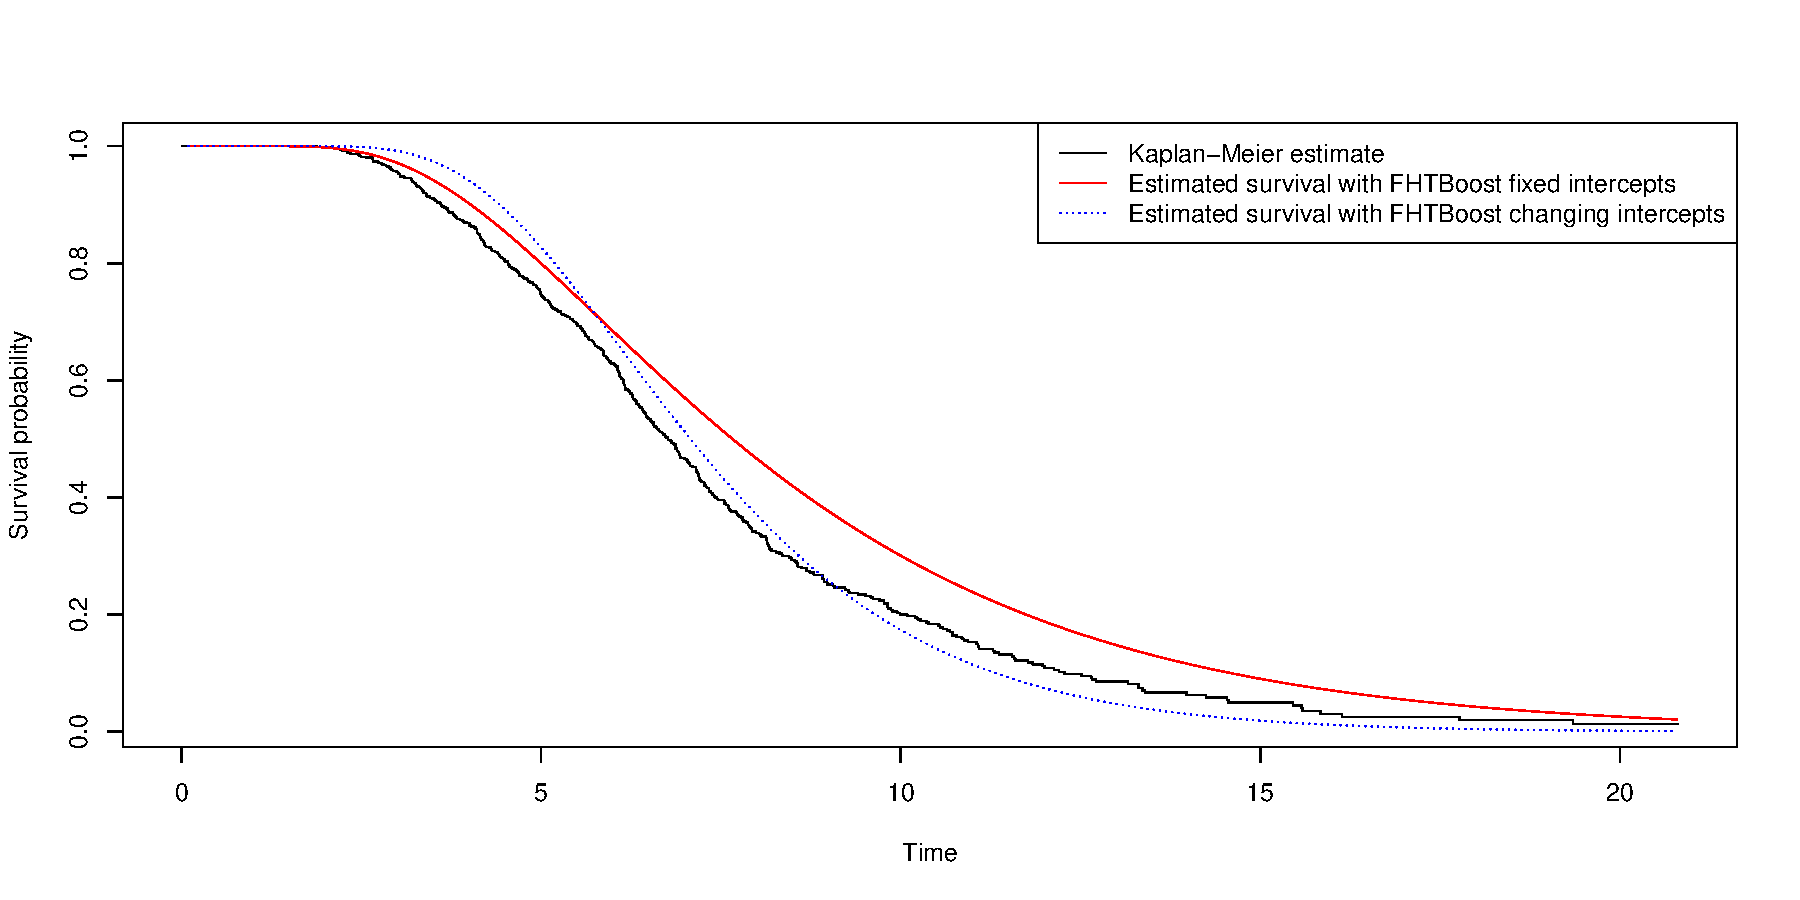
\includegraphics[scale=0.4]{figures/kaplan_meier_small.pdf}
\end{figure}
We estimate $\hat{\bbeta}$ and $\hat{\bgamma}$ using FHTBoost, which we in this case run until convergence.
\begin{figure}
\caption{Negative log-likelihood for the boosting algorithm with both fixed and changing intercept, as a function of iteration number $m$}
\label{fig:boosting-ML}
\centering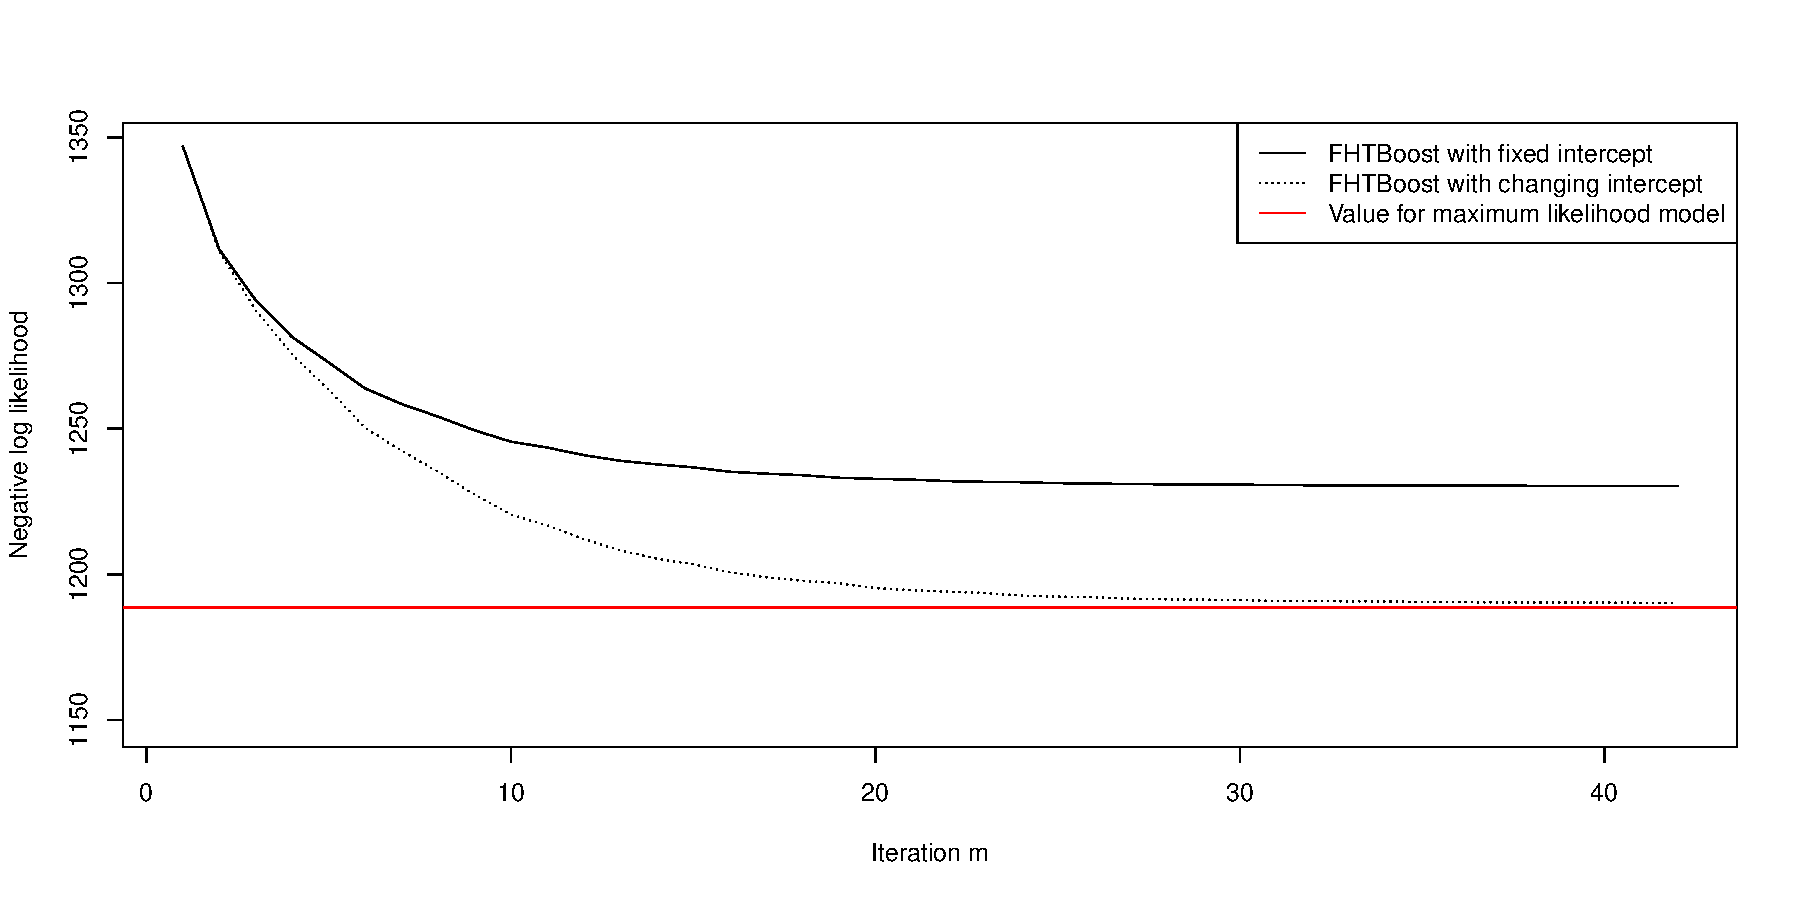
\includegraphics[scale=0.4]{figures/small_example.pdf}
\end{figure}
Figure \ref{fig:boosting-ML} shows a plot of the negative log likelihood of the data (training error) as a function of the iteration number $m$.
The solid black line shows negative log-likelihood for FHTBoost with a fixed intercept, i.e. Algorithm \ref{algo:fhtboost}.
In this version with fixed intercept, we only estimate the intercepts $\hat{\boldeta}_0=\left(\hat{\beta}_{0},\,\hat{\gamma}_{0}\right)$ before we begin iterating, and so these intercepts are not changed in any of the boosting iterations.
The horizontal solid red line shows the negative of the maximum likelihood, obtained through numerical maximization of the joint maximum likelihood.
It is clear that FHTBoost with a fixed intercept does not reach the maximum likelihood value.
The maximum likelihood estimated intercepts are $\hat{\beta}^{\text{ML}}_{1,0}=1.98$ and $\hat{\beta}^{\text{ML}}_{2,0}=-1.02$.
FHTBoost with a fixed intercept produces estimates of the intercepts as $\hat{\beta}_{0}=1.68$ and $\hat{\gamma}^{[\mstop]}_{0}=-0.71$.
These estimated intercepts are quite off from the maximum likelihood estimates (see also Table \ref{table:ML}).

To achieve the maximum likelihood value, we found out that we have to modify the algorithm to change intercepts while boosting.
Some existing boosting algorithms modify the intercept, but we fount it unclear in the literature how these perform it.
\textit{mboost} uses linear least squares base learners with an intercept \citep{mboost}.
One way to change the intercept in each boosting iteration is to treat is as a nuisance parameter, i.e. perform numerical maximization after updating the additive predictor.
This will be the same as is done initially to find the intercepts, except now we are using the estimated additive predictors as offsets.
Since we will change intercepts in each iteration, we now denote intercepts with their iteration number as well.
We write $\hat{\beta}_{0}^{[m]}$ and $\hat{\gamma}_{0}^{[m]}$.
The initial intercepts are then $\hat{\beta}_{0}^{[0]}$ and $\hat{\beta}_{0}^{[0]}$.
We replace these in each iteration, with $\hat{\beta}_{0}^{[m]}$ and $\hat{\beta}_{0}^{[m]}$, which are calculated in the intercept estimated in step $m$ of the boosting algorithm.
By incorporating \textit{changing} intercepts, the algorithm was successful in recovering the maximum likelihood value and parameters.
See table \ref{table:ML} for the estimated parameter values, and graphically, in figure \ref{fig:boosting-ML}, where the convergence is plotted as a function of the number of boosting iterations.
\begin{table}\caption{Parameter values for the example in subsection \ref{subsec:algo-example}}
\label{table:ML}
\centering
\begin{tabular}{lcccccc}
\toprule
    & $\hat{\beta}_{0}$ & $\hat{\beta}_{1}$ & $\hat{\beta}_{2}$ & $\hat{\gamma}_{0}$ & $\hat{\gamma}_{1}$ & $\hat{\gamma}_{2}$ \\
\hline
Maximum likelihood estimate                   &    1.98 &    0.10 &    0.21 &    -1.03 &    -0.09 &     0.12 \\
FHTBoost with fixed intercept                 &    1.68 &    0.10 &    0.18 &    -0.72 &    -0.06 &     0.09 \\
FHTBoost with changing intercept              &    1.97 &    0.10 &    0.18 &    -1.02 &    -0.09 &     0.12 \\
\bottomrule
\end{tabular}
\end{table}
When we update the intercept in each iteration the final model has the interpretation that the resulting intercepts are the maximum likelihood intercepts \textit{including} the covariate effects estimated while boosting.
Meanwhile, for the fixed intercept, the estimated intercepts are the maximum likelihood intercepts \textit{without} estimated covariate effects.

\section{FHTBoost algorithm with changing intercept}\label{subsec:FHT-intercept}
%\begin{algorithm}
We modify algorithm \ref{algo:fhtboost} with the proposed modification with changing the intercepts in each iteration.
We replace step \ref{algostep:FHT-end} in the fixed intercept algorithm, where we now incorporate changing intercepts for the additive predictors in each boosting iteration.
See Algorithm \ref{algo:fhtboost-with-intercept} for a schematic overview of this change.
Note that while this version of the algorithm did lead to reaching the maximum likelihood value on the simulated example, it is not necessarily better to use this than the fixed intercept version.
Since we treat the intercept as a nuisance parameter, there is a risk of overfitting by changing the intercept too much.
After all, we are interested in the additive predictors which minimize the test error, not the training error.
In fact, as we will see in the simulation study in a later chapter, the fixed intercept version performs worse than the changing intercept version.
In the next chapter, we will introduce and explain evaluation measures which we will use to evaluate the performance of FHTBoost.

\begin{algorithm}
\caption{FHTBoost with fixed intercept}
\label{algo:fhtboost-with-intercept}
\begin{enumerate}
    \setcounter{enumi}{6}
    \item
        Find which parameter should be included in the model,
        \begin{equation*}
            k^{[m]}=\argmin_{k\in\{1,2\}}\Delta\rho_k.
        \end{equation*}
        Include this component in the final model, by updating its additive predictor,
        \begin{equation*}
            \hat{\eta}^{[m]}_{k^{[m]}}=\hat{\eta}^{[m-1]}_{k^{[m]}}+\nu\cdot\hat{h}^{[m]}_{k^{[m]},\,j^{[m]}}(x),
        \end{equation*}
        while for the other component $k\neq k^{[m]}$, set the additive predictor for this iteration to be the same as previous iteration
        \begin{equation*}
            \hat{\eta}^{[m]}_{k}=\hat{\eta}^{[m-1]}_{k}.
        \end{equation*}
        Now, update the intercepts $\hat{\beta}_0$ and $\hat{\gamma}_0$ in the additive predictors by maximizing the training error with the other parts of the estimated additive predictors as offsets.
        The new offsets are thus
        \begin{equation*}
            \left(\beta_0^{[m]},\gamma_0^{[m]}\right)=\argmin_{\left(\beta_0,\gamma_0\right)}
            \err
                \left(
                    \left(
                        \beta_0,\beta^{[m]}_1,\ldots,\beta^{[m]}_{p_1}
                    \right),
                    \left(
                        \gamma_0,\gamma^{[m]}_1,\ldots,\gamma^{[m]}_{p_2}
                    \right)
                \right)
        \end{equation*}
        Here each $\beta_j^{[m]}$ is the sum of the shrunk estimated parameters so far, i.e.,
        \begin{equation*}
            \hat{\beta}_j^{[m]}=\sum_{a=1}^{m}\nu\cdot\indicator\left(j_1^{[a]}=j\right)\hat{\beta}_j^{[a]},
        \end{equation*}
        and similarly for $\gamma_j^{[m]}$.
\end{enumerate}
\end{algorithm}